%%
%% Ring Counters - A crash introduction on Ring Counters
%% University of Applied Sciences, Electrical Engineering.
%%
%% (c)2015, J. op den Brouw <J.E.J.opdenBrouw@hhs.nl>
%% v0.1
%%
%% This document is created for the benefit of the students who
%% follow the project course PRO-P2, the end project of the first
%% year of the study program Electrical Engineering.
%%


%% 12pt charachters, A$ paper size, one side printing, equation left aligned
%% equation indent at 1 em
\documentclass[12pt,a4paper,final,twoside,fleqn]{article}
\setlength{\mathindent}{1em}

%% PDF Version and compression...
\pdfminorversion=5
\pdfobjcompresslevel=2

%https://www.ctan.org/pkg/inputenc
%% Set input encoding to ISO-8859-1 (latin1)
\usepackage[utf8]{inputenc}
%% Use T1 output font encoding
\usepackage[T1]{fontenc}

%% Dutch spelling of chapter, section, etc.
%% http://ftp.snt.utwente.nl/pub/software/tex/macros/latex/required/babel/base/babel.pdf
\usepackage[english]{babel}
%% http://ctan.cs.uu.nl/macros/latex/contrib/csquotes/csquotes.pdf
\usepackage{csquotes}

%% Set page layout
%% http://ctan.cs.uu.nl/macros/latex/contrib/geometry/geometry.pdf
\usepackage[a4paper,bindingoffset=0.2in,left=1in,right=1in,top=1in,bottom=1.4in,footskip=0.6in]{geometry}

%% Parskip et al.
%% http://ctan.cs.uu.nl/macros/latex/contrib/parskip/parskip-doc.pdf
\usepackage{parskip}

%% Include graphics files
%% http://ctan.cs.uu.nl/macros/latex/required/graphics/grfguide.pdf
\usepackage{graphicx}

%% Customizing lists
%% http://ctan.cs.uu.nl/macros/latex/contrib/enumitem/enumitem.pdf
\usepackage{enumitem}

%% Use the AMS Mathematical typesetting
%% http://ctan.cs.uu.nl/macros/latex/contrib/mathtools/mathtools.pdf
\usepackage{mathtools}
\usepackage{amsfonts}
\usepackage{amssymb}

%% Define and use colors
%% http://ctan.cs.uu.nl/macros/latex/contrib/xcolor/xcolor.pdf
\usepackage{xcolor}

%% Use the Latin Modern font...
%% https://www.ctan.org/tex-archive/fonts/lm
\usepackage{lmodern}

%% Subliminal refinements towards typographical perfection
%% http://ctan.cs.uu.nl/macros/latex/contrib/microtype/microtype.pdf
\usepackage[stretch=10]{microtype}

%% Default monospaced font from inconsolata, e.g. for listings
%% http://ctan.cs.uu.nl/fonts/inconsolata/doc/inconsolata-doc.pdf
\usepackage[scaled=0.90]{inconsolata}

%% http://ctan.cs.uu.nl/macros/latex/contrib/biblatex/doc/biblatex.pdf
%% neem paginanummer niet samen in de backref lijst dus 1,2,3 i.p.v. 1-3 (anders kun je niet op 2 klikken)
\usepackage[
    backend=biber,
    backref=true,
    backrefstyle=none,
    sortcites=true,
    sorting=none,
    doi = false % doi informatie wordt niet weergegeven
]{biblatex}
\addbibresource{bibliography.bib}
\DefineBibliographyStrings{dutch}{
    backrefpage = {blz.},
    backrefpages = {blz.},
}

%% http://ctan.cs.uu.nl/macros/latex/contrib/titlesec/titlesec.pdf
% Verander opmaak titels
\newcommand{\sectionfont}{\rmfamily\bfseries}
\newcommand{\headerfont}{\rmfamily\small}
\newcommand{\footerfont}{\rmfamily\small}
\usepackage{titlesec}
\titleformat{\section}{\sectionfont\large}{\thesection}{1em}{}
\titleformat{\subsection}{\sectionfont\large}{\thesubsection}{1em}{}
\titleformat{\subsubsection}{\sectionfont}{\thesubsubsection}{1em}{}
\titlespacing*{\section}{0pt}{\baselineskip}{\aftersubsection}
\newlength{\aftersubtitle}
\setlength{\aftersubtitle}{1.2\baselineskip}
\newlength{\aftersubsection}
\setlength{\aftersubsection}{\aftersubtitle}
\addtolength{\aftersubsection}{-\baselineskip}
\titlespacing*{\subsection}{0pt}{.8\baselineskip}{\aftersubsection}
\titlespacing*{\subsubsection}{0pt}{.6\baselineskip}{0pt}

% http://archive.cs.uu.nl/mirror/CTAN/macros/latex/contrib/footmisc/footmisc.pdf
% ruimte onder aan de pagina tussen tekst en voetnoot niet na voetnoot
% package moet VOOR fancyhdr om warning te voorkomen
\usepackage[
    bottom,
    hang,
    multiple
]{footmisc}
% inspringen
\setlength{\footnotemargin}{1em}
% ruimte tussen footnotes:
\setlength{\footnotesep}{.8\baselineskip}

%% Making captions nicer...
%% http://ctan.cs.uu.nl/macros/latex/contrib/caption/caption-eng.pdf
\usepackage[font=footnotesize,format=plain,labelfont=bf,up,textfont=it,up]{caption}

%% Using hyperrefs...
%% http://ctan.cs.uu.nl/macros/latex/contrib/hyperref/hyperref.pdf
\usepackage{hyperref}
\hypersetup{
	colorlinks=true,
	linkcolor=blue,
    pdftitle={An Introduction to Ring Counters},    % title
    pdfauthor={J.E.J. op den Brouw},     % author
    pdfsubject={A crash course on Ring Counters},   % subject of the document
    %pdfcreator={Latex},   % creator of the document
    %pdfproducer={PDFtoLaTex}, % producer of the document
    pdfkeywords={digital design} {counter} {ring counter} {Johnson counter} % list of keywords
}

%% Use computer code listings
%% http://ctan.cs.uu.nl/macros/latex/contrib/listings/listings.pdf
\usepackage{listings}
%% Need textcomp for upquotes
%% https://www.ctan.org/pkg/textcomp
\usepackage{textcomp}

%%% No package loading from here

%% The title page
\makeatletter
\def\maketitle{%
  \null
  \thispagestyle{empty}%
  \vskip 3cm
  \begin{center}\leavevmode
    {\LARGE \@title\par}%
    \vskip 1cm
    {\large \@author\par}%
    \vskip 0.03cm
    {\large The Hague University of Applied Sciences\par}%
    \vskip 0.03cm
    {\large \@date\par}%
  \end{center}%
  \vfill
  \null
}
\makeatother

%% Author's credentials
\author{Jesse op den Brouw}
\title{An Introduction to Ring Counters}
\date{\today}

%% Some colours
\definecolor{gray}{rgb}{0.5,0.5,0.5}
\definecolor{lightgray}{rgb}{0.95,0.95,0.95}

%% Set the typesetting of VHDL files
\lstset{ %
  language=VHDL,                        % the language of the code
  basicstyle=\footnotesize\ttfamily,    % the size of the fonts that are used for the code
  numbers=left,                         % where to put the line-numbers
  numberstyle=\tiny\color{gray},        % the style that is used for the line-numbers
  stepnumber=1,                         % the step between two line-numbers. If it's 1, each line will be numbered                           
  numbersep=8pt,                        % how far the line-numbers are from the code
  backgroundcolor=\color{lightgray},    % choose the background color. You must add \usepackage{color}
  showspaces=false,                     % show spaces adding particular underscores
  showstringspaces=false,               % underline spaces within strings
  showtabs=false,                       % show tabs within strings adding particular underscores
  frame=lines,                          % adds framing around the code
  rulecolor=\color{black},              % if not set, the frame-color may be changed on line-breaks within not-black text (e.g. comments (green here))
  tabsize=4,                            % sets default tabsize to 4 spaces
  captionpos=b,                         % sets the caption-position to bottom
  breaklines=true,                      % sets automatic line breaking
  breakatwhitespace=false,              % sets if automatic breaks should only happen at whitespace
  title=\lstname,                       % show the filename of files included with \lstinputlisting;
  upquote=true,
}

%% Nice overbar in Boolean equations
\newcommand*{\oline}[1]{\overline{#1\mathstrut}}

%% Ahhhh... At last, the beginning of the document...
\begin{document}

%% Make title page
\maketitle
\begin{abstract}
\noindent
Ring counters are a type of counters composed of shift registers. They are extremely
fast and require few logic gates. This document introduces two types of ring counters,
the straight ring counter and the Johnson counter. The latter is elaborated on in
detail. Some applications are described as well as commercially available devices
and designs using Johnson counters. A generic VHDL description and a description of
the commercially available 4017 are provided.
\end{abstract}
\vspace*{2cm}

%% Make table of contents
\clearpage
\renewcommand\contentsname{Table of Contents}
\tableofcontents
\vspace{1cm}
\listoffigures
\vspace{1cm}
\renewcommand{\lstlistlistingname}{List of Listings}
\lstlistoflistings
\vfill
{\small
Any questions or comments regarding this document can be sent to
\href{mailto:J.E.J.opdenBrouw@hhs.nl}{J.E.J.opdenBrouw@hhs.nl}
}
\clearpage


\section{Ring Counters}
Ring counters are a type of counter created using \textsl{shift registers}. A shift
register is constructed using D-type flip-flops where the output of one flip-flop
is connected to the input of another flip-flop~\cite{morrismano2006}. With ring
counters, the output of the last flip-flop is fed to the input of the first flip-flop.
Ring counters do not count using normal binary code, but their internal state can be
used to decode to any output sequence wanted.

There are two types of ring counters:

\begin{enumerate}[label={\alph*})]
 \item Straight ring counter
 \item Johnson counter
\end{enumerate}

There is a third counter type using a shift register, the Linear Feedback Shift
Register (LFSR). It has a more elaborate feedback circuit than the other two ring
counters and is therefore not discussed in this document.


\section{Straight ring counter}
A straight ring counter or Overbeck counter connects the output of the last
flip-flop to the first flip-flop input and circulates a single one bit around
the ring. It provides a \textsl{one-hot} counting sequence. For example, in a
4-register ring counter, with initial register values of 1000, the repeating
sequence is 1000, 0100, 0010, 0001. Note that one of the flip-flops must be
pre-loaded with a logic 1 in order for it to operate properly. Also note that
an $n$-bit ring counter cycles through exactly $n$ states.

A schematic of a 4-bit straight ring counter is given in
Figure~\ref{fig:straightringcounter}. The asynchronous reset will set the
initial contents of the counter to 1000 (note that the least significant
flip-flop is on the left side).

\begin{figure}[h!]
  \centering
  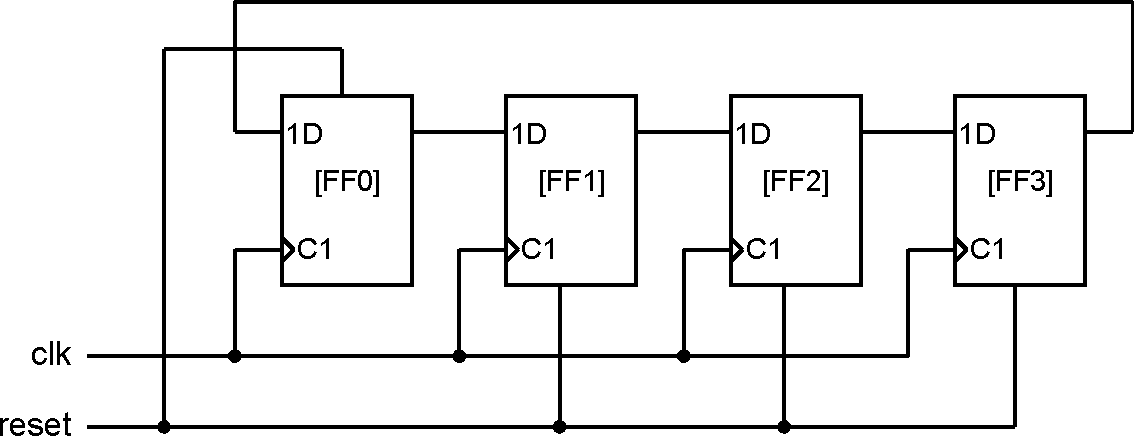
\includegraphics[scale=0.60]{straightringcounter_4bit}
  \caption[A 4-bit straight ring counter]{A 4-bit straight ring counter.}
  \label{fig:straightringcounter}
\end{figure}

Straight ring counters are currently seldom used and there are no commercial
devices available. In the past, they were mainly used as decimal counters using
\textsl{Nixie tubes} and \textsl{neon tubes}~\cite{manley1950,dekker2015}.


\section{Johnson Counter}
Another form of ring counter is created by feeding back the complement of the contents
of the last flip-flop to the input of the first flip-flop. This is called a
\textsl{twisted ring counter}, but is better known as the \textsl{Johnson counter}.
The alternative term M\"obius counter is found in many books and articles because
the Johnson counter resembles the famous M\"obius strip~\cite{wiki2015a}. For example,
in a 5-flip-flop Johnson counter with an initial register contents (or state) of 00000,
the repeating sequence is 00000, 10000, 11000, 11100, 11110, 11111, 01111, 00111, 00011,
00001. When observing the pattern, it can be seen that any changes between succeeding
states, only one flip-flop changes state. As a result, any of these states is directly,
spike-free decodable with only a two-input
% Need mbox otherwise the reference number will split across lines
\mbox{gate~\cite{brcic1965,asicdigitaldesign2015}.}

Figure \ref{fig:johnsoncounter} shows a 5-bit Johnson counter with \textsl{terminal
count} output \lstinline|tc|. This output becomes high in the last counting state 00001
before returning to 00000.

\begin{figure}[h!]
  \centering
  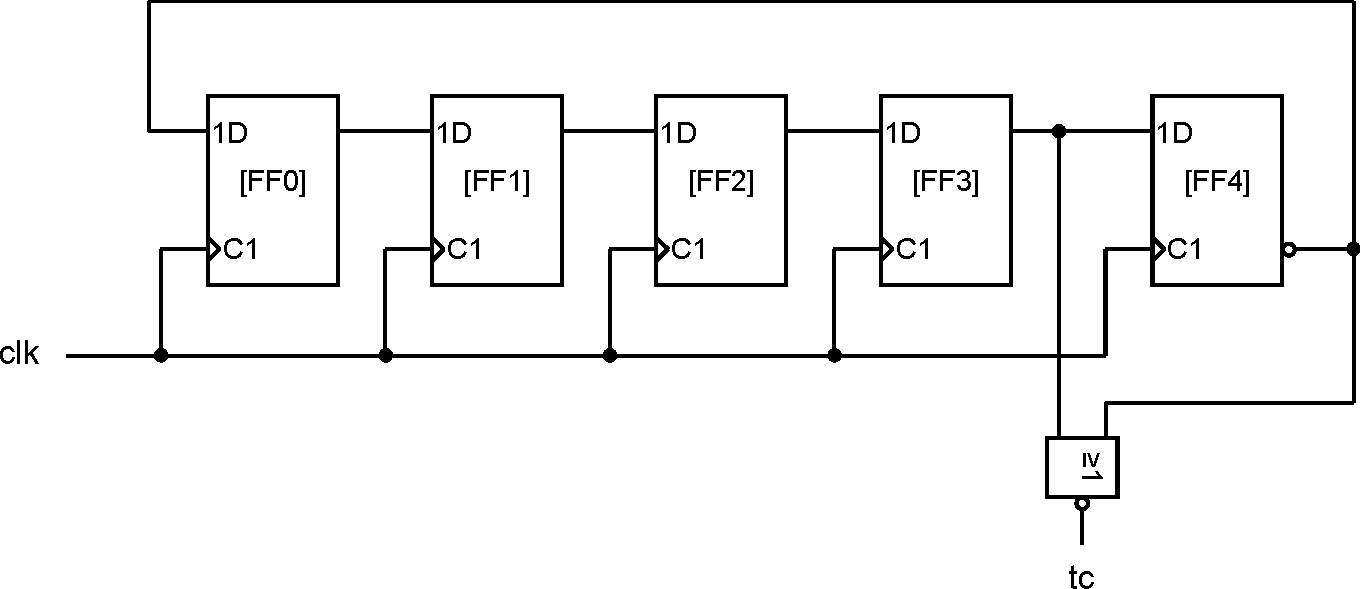
\includegraphics[scale=0.60]{johnson_5bit}
  \caption[A 5-bit Johnson Counter with Terminal Count]{A 5-bit Johnson Counter
           with Terminal Count. The reset is omitted for clarity.}
  \label{fig:johnsoncounter}
\end{figure}

Only the two most significant flop-flops have to be sampled, so $tc$ is logic
`1' when $Q_3$ is logic `0' and $Q_4$ is logic `1'. Using De Morgan's theorem,
the resulting function can be realised using a NOR gate and the already 
available flip-flop outputs.
%
\begin{equation}
tc = \oline{Q_3} \cdot Q_4 = \oline{Q_3 + \oline{Q_4}}
\end{equation}
%
It can be easily shown that an $n$-bit Johnson counter cycles through exactly
$2n$ states. This becomes increasingly inefficient for $n>2$ since any $n$-bit
counter has $2^n$ states by itself. If the Johnson counter enters a state that
does not belong to the original counting sequence, it will exhibit a single
\textsl{parasitic counting sequence} with $2^n - 2n$
states~\cite{zwolinski2004,wilson2011}. This is why most commercial devices
incorporate \textsl{self-correcting} logic. Within a full counting sequence or
so, the device will resume normal operation, as shown for example in the
schematic in~\cite{datasheetcd4017b}.

Johnson counters are very fast because there is no logic between the output of
one flip-flop and the input of another flip-flop, i.e., there is no next state
logic (one would expect an inverter in the feedback loop but the inverted
output of a flip-flop is usually available, especially on
ASIC's~\cite{weste2011}). Therefore the maximum frequency at which the counter
operates reliably is given by~\eqref{equ:freqjohn}.
%
\begin{equation}
\label{equ:freqjohn}
f_{max} = \dfrac{1}{t_{P(max)}(\mathrm{FF}) + t_{su}(\mathrm{FF})}
\end{equation}
%
where $f_{max}$ is the maximum obtainable frequency, $t_{P(max)}(\mathrm{FF})$
is the maximum propagation delay of the flip-flop outputs with respect to
the active clock edge and $t_{su}(\mathrm{FF})$ is the setup time of the
flip-flops. The propagation delay of output \lstinline|tc| with respect to
the active clock edge is given by~\eqref{equ:tpmaxtc}.
%
\begin{equation}
\begin{split}
\label{equ:tpmaxtc}
t_{P(max)}(\mathrm{tc}) &= t_{P(max)}(\mathrm{FF}) + t_{P(max)}(\mathrm{NOR}) \\
t_{P(min)}(\mathrm{tc}) &= t_{P(min)}(\mathrm{FF}) + t_{P(min)}(\mathrm{NOR}) \\
\end{split}
\end{equation}
%
where $t_{P(min)}$ and $t_{P(max)}$ are the minimum and maximum propagation
delays of the named signals.


\section{Applications of Johnson counters}
A 5-stage Johnson counter can be used as a decade frequency
divider~\cite{marston1996}.

Johnson counters are used as multiphase clock signal generators. Such
generators are used in large digital systems where timing signals are needed
with high accuracy with respect to the central clock~\cite{thijssen2000}.
Johnson counters produce glitch free symmetric (50\% duty cycle) outputs per
count cycle~\cite{cohen2002}. A good example is given by Harris~\cite{harris2002}.

Amann et al.~\cite{amann1988} have shown that designing FSMs using loadable
Johnson counters as state memory saves up to 30\% of the product terms
generating the next state and outputs.

Johnson counters are used to drive stepper motor
circuits~\cite{linfw1975,allaboutcircuits2015}.


\section{Commercially available Johnson counters}
The CD4017B is an all-CMOS, commercially available 5-stage Johnson counter with
decoded outputs~\cite{datasheetcd4017b}. It is used in a wide variety of designs,
mostly as a 10-stage counter (counting to 10 is done as long as mankind exists).
The device is very popular and cheap but it has a big design flaw: clock gating.
The \lstinline|clock| signal is AND-gated with the \lstinline|clock_inhibit|
signal. It produces pulse-triggered behaviour of the clock input
(\lstinline|clock_inhibit| must be held stable when \lstinline|clock| is high) and
exhibits clock skew (the resulting clock pulse is delayed by the AND gate). Note
that the internal shift register contents is not available on output pins, only the
ten decoded outputs are available making the 4017 behave as a straight ring counter. 

The CD4022B is essentially a 4-stage version of the 4017~\cite{datasheetcd4022b}.

The 70HC/HCT4017 is a 7400 remake of the 4017. The HCT has TTL compatible power
supply, inputs and outputs.


\section{Design using Johnson Counters}
A very nice design using Johnson counters is the LFO generator by R.G. Keen~\cite{keen2015}.

A number of 4017 designs, including an automatic bathroom light switch and a
led chaser circuit, can be found on~\cite{electroschematics2015}.

Using a number of 4017, one can build a Nixie tube digital clock~\cite{harrison2015}.

The 4026 and 4033 Decade Counters consist of a 5-stage Johnson counter similar
to the 4017 and an output decoder that converts the counter state to 7-segment
decoded outputs~\cite{datasheetcd4026b}.

Ben Kuiper describes a range detection circuit using 4017's (and more 4000-series 
devices) in~\cite{kuiper2015}.


\section{VHDL description of a Johnson counter}
Describing a Johnson counter in VHDL is easy and straightforward. Using the schematic
of Figure~\ref{fig:johnsoncounter}, the entity in Listing~\ref{cod:johnson} consists
of a clock input, an asynchronous reset input, a count output and a terminal count
output.

The counter is set to all zeros when the reset input is high. The rising edge is chosen
as active clock edge. On the rising edge of the clock the contents of the register is
shifted one stage towards the most significant flip-flop and the least significant
flip-flop is loaded with the complement of the most significant flip-flop. This is done
using standard VHDL implementation with the \lstinline|&| concatenation operator.

This implementation makes use of so-called \textsl{generic constants}. The design is
written as an $n$-stage Johnson counter. During instantiation, the generic constant
$n$ has to be supplied as a positive number. When absent, the design is instantiated
with $n=5$.

\medskip
\begin{lstlisting}[caption=A VHDL description of an n-stage Johnson counter,label=cod:johnson]
-- Filename:     johnson_counter.vhd
-- Filetype:     VHDL Design Unit
-- Date:         5 mar 2015
-- Update:       -
-- Description:  VHDL Description of a n-stage Johnson Counter
-- Author:       J. op den Brouw
-- State:        Demo
-- Error:        -
-- Version:      1.0
-- Copyright:    (c)2015, De Haagse Hogeschool

-- This VHDL description describes the behaviour of n-stage
-- Johnson counter with spike free active high decoded terminal
-- count output.

-- Using the 1164 std_logic
library ieee;
use ieee.std_logic_1164.all;

-- Tbe port description of the Johnson counter
entity johnson_counter is
    generic (n : integer := 5);
    port (clk :    in std_logic;
          areset : in std_logic;
          count :  out std_logic_vector (0 to n-1);
          tc :     out std_logic
         );
end entity johnson_counter;

architecture rtl of johnson_counter is
-- Internal counter signal
signal count_int : std_logic_vector (0 to n-1);
begin

    -- The Johnson counter itself
    process (clk, areset) is
    begin
        -- The reset is active high
        if areset = '1' then
            -- Set all counter bits to 0, nice VHDL trick
            count_int <= (others => '0');
        elsif rising_edge(clk) then
            -- Shift the lot a stage and feed back the last one
            count_int <= not count_int(n-1) & count_int(0 to n-2);
        end if;
    end process;
    
    -- The outputs
    count <= count_int;
    -- tc high when counter is ...01, where the dots should be all zeros.
    -- tc <= (not count_int(n-1)) nor count_int(n-2);
    -- tc <= '1' when count_int(n-1) = '1' and count_int(n-2) = '0' else '0';
    tc <= '1' when count_int(n-2 to n-1) = "01" else '0';
	 
end architecture rtl;
\end{lstlisting}


\section{The 4017 in VHDL}
In Listing~\ref{cod:cd4017b}, a VHDL description of the 4017 Johnson counter is
presented. The description is created using the schematic in~\cite{datasheetcd4017b}.
There is one omission: in the original design, the clock input has a Schmitt-trigger
input.

\medskip
\begin{lstlisting}[caption=A VHDL description of the 4017 5-stage Johnson counter,label=cod:cd4017b]
-- Filename:     cd4017b.vhd
-- Filetype:     VHDL Design Unit
-- Date:         5 mar 2015
-- Update:       -
-- Description:  VHDL Description of a CD4017B 5-stage Johnson Counter
-- Author:       J. op den Brouw
-- State:        Demo
-- Error:        -
-- Version:      1.0
-- Copyright:    (c)2015, De Haagse Hogeschool
--
-- This VHDL description describes the behaviour of an CD4017B 5-stage
-- Johnson counter with spike free active high decoded outputs.
-- See http://www.ti.com/lit/ds/symlink/cd4017b.pdf for more information.
--
-- In some designs, the naming of the pins is different:
--      clock -> CP0
--      clock_inhibit -> ~CP1   or    not(CP1)
--      reset -> MR
--      carry out -> not(Q)5--9
--
-- Please note that this design uses clock-gating: the clock is gated
-- with an AND gate and a signal clock_inhibit. This is a poor hardware
-- design. It produces both pulse-triggered behaviour of the clock input
-- (clock_inhibit must be held stable when clock is high) and clock skew
-- (the resulting clock pulse is delayed by the AND gate).
-- PLEASE USE THIS DESIGN FOR REFERENCE ONLY, NOT IN REAL PRODUCTS.

-- Using the 1164 std_logic
library ieee;
use ieee.std_logic_1164.all;

-- The port description of the 4017
entity cd4017b is
    port (clock :         in std_logic;
          reset :         in std_logic;
          clock_inhibit : in std_logic;
          q :             out std_logic_vector (9 downto 0);
          carry_out :     out std_logic
	     );
end entity cd4017b;

architecture gate_level of cd4017b is
-- In the datasheet, FF1 is on the left side
signal count_int : std_logic_vector (1 to 5);
-- Internal signal for clock gating
signal clk_int : std_logic;
begin
    -- The clock is gated
    clk_int <= (not clock) nor (not (not clock_inhibit));

    -- The Johnson counter itself
    process (clk_int, reset) is
    begin
        if reset = '1' then
            count_int <= "00000";
        elsif rising_edge(clk_int) then
            count_int(5) <= count_int(4);
            count_int(4) <= count_int(3);
            count_int(3) <= not (((not count_int(1)) and (not count_int(3))) or
                                  (not count_int(2)));
            count_int(2) <= count_int(1);
            count_int(1) <= not count_int(5);
        end if;
	 end process;

	 -- The outputs
	 carry_out <= not count_int(5);
	 q(0) <= not (not count_int(1) nand not count_int(5));
	 q(1) <= not (    count_int(1) nand not count_int(2));
	 q(2) <= not (    count_int(2) nand not count_int(3));
	 q(3) <= not (    count_int(3) nand not count_int(4));
	 q(4) <= not (    count_int(4) nand not count_int(5));
	 q(5) <= not (    count_int(1) nand     count_int(5));
	 q(6) <= not (not count_int(1) nand     count_int(2));
	 q(7) <= not (not count_int(2) nand     count_int(3));
	 q(8) <= not (not count_int(3) nand     count_int(4));
	 q(9) <= not (not count_int(4) nand     count_int(5));
	 
end architecture gate_level;\end{lstlisting}

% Add bibliography to toc with clickable reference
\phantomsection
\addcontentsline{toc}{section}{\refname}
\printbibliography{}

\end{document}